Betrachten Sie die Differentialgleichung
\begin{equation}
\frac{dx}{dt}
=
x^4-4x^2-\lambda
\label{aufgabe301:gl}
\end{equation}
\begin{teilaufgaben}
\item
Finden Sie die Gleichgewichtslösungen und untersuchen Sie die 
Bifurkationen, die bei Veränderungen des Parameters $\lambda$
auftreten können.
\item
Welche Gleichgewichtslösung wird das System einnehmen, wenn der
Parameter $\lambda$ erst von $-1$ auf $1$ anwächst
und dann wieder auf $-1$ absinkt.
\end{teilaufgaben}

\begin{loesung}
\begin{figure}
\centering
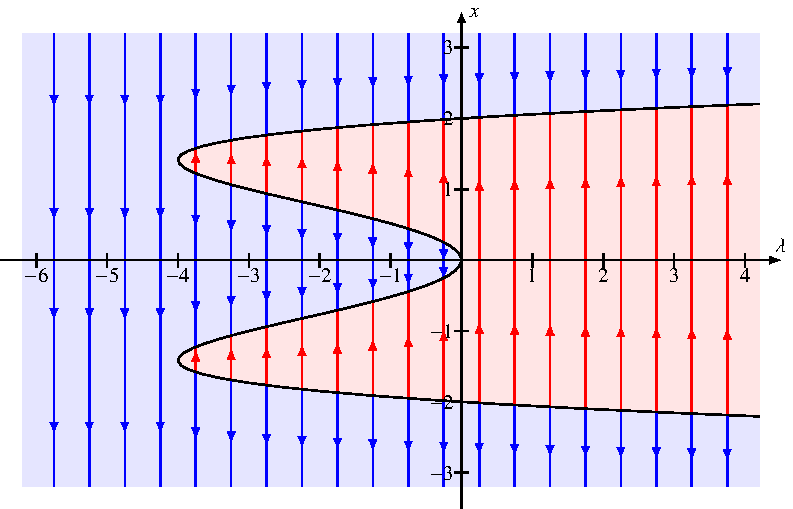
\includegraphics{chapters/3/grad4.pdf}
\caption{Phasendiagramm der Differentialgleichung~\eqref{aufgabe301:gl}.
\label{aufgabe301:fig}}
\end{figure}
\begin{teilaufgaben}
\item
Die kritischen Punkte der Differentialgleichung~\eqref{aufgabe301:gl}
sind Nullstellen der Gleichung
\begin{equation}
x^4-4x^2-\lambda=0
\label{aufgabe301:nullstellen}
\end{equation}
Dies ist eine quadratische Gleichung in $x^2$, die mit der Lösungsformel
für die quadratische Gleichung gelöst werden kann:
\[
x^2 = 2 \pm \sqrt{4+\lambda}.
\]
Diese Gleichung hat reelle Lösungen für $\lambda \ge -4$.
Für $\lambda \le 0$ ist die Quadratwurzel nicht grösser als $2$,
so dass die beiden Nullstellen positiv sind, es also vier verschiedene
Lösungen
\begin{equation}
x_{1,2,3,4} = \pm\sqrt{2\pm\sqrt{4+\lambda}}
\end{equation}
hat.
Für $\lambda >0$ hat die quadratische Gleichung eine negative Lösung
für $x^2$, die also nicht zu einer reellen Lösung der
Gleichung~\eqref{aufgabe301:nullstellen} führen kann.
Nur aus der positive Lösung $2+\sqrt{4+\lambda}$ kann man eine
Gleichgweichslösung, nämlich
\[
x=\pm\sqrt{2+\sqrt{4+\lambda}}
\]
ableiten.
Für $\lambda < -4$ gibt es gar keine Gleichgewichtslösung.

Das Phasendiagramm in Abbildung~\ref{aufgabe301:fig} zeigt,
dass für $\lambda >0$ die obere Gleichgewichtslösung stabil ist,
untere dagegen instabil.
Für $-4\le\lambda\le 0$ sind die Gleichgewichtslösungen
\begin{align*}
&\sqrt{2+\sqrt{4+\lambda}}
&&\text{und}&
&-\sqrt{2-\sqrt{4+\lambda}}
\\
\intertext{stabil und die Gleichgewichtslösungen}
&-\sqrt{2+\sqrt{4+\lambda}}
&&\text{und}&
&\sqrt{2-\sqrt{4+\lambda}}
\end{align*}
instabil.

Bei $\lambda=-4$ finden gleichzeitig zwei Sattel-Knoten-Bifurkationen 
statt, bei $\lambda=0$ findet ein einfache Sattel-Knoten-Bifurkation
statt, jedoch in umgekehrter Richtung wie im Beispiel im Text.
\item
Beim Anwachsen des Parameters über den Punkt $\lambda=0$ springt die
Gleichgewichtslösung auf die stabile Lösung
\[
x(\lambda)=\sqrt{2+\sqrt{4+\lambda}}.
\]
Bei der anschliessenden Verringerung von $\lambda$ bleibt die 
Gleichgewichtslösung auf dem Ast $x(\lambda)$ der Kurve, da diese
alle stabil sind.
Unabhängig vom Ausgangszustand befindet sich das System am Ende des
beschriebenen Szenarios also immer in der Nähe der Gleichgewichtslösung
\[
x(-1)=\sqrt{2+\sqrt{3}}.
\qedhere
\]
\end{teilaufgaben}
\end{loesung}

